\clearpage
\setcounter{page}{1}
\maketitlesupplementary
% Comparison of accuracy (%) on ImageNet-C (level 5) with pairwise collaboration of all models
% In the supplementary materials, we provide additional experimental results and further details of our proposed approach, COCA. 
% We also explore the applicability of COCA across multiple models. 
\appendix
\section{Pseudo-code of COCA}
\label{pscode}
\begin{algorithm}
\begin{spacing}{1.1}
\caption{The pipeline of proposed COCA.}
\label{alg:coca}
\textbf{Input:} Test samples $D^{\text{test}}=\{x_j\}_{j=1}^M$, the pre-trained models $f_{\theta_{1}}, f_{\theta_{2}}$ with trainable parameters $\widetilde{\theta}_{1}, \widetilde{\theta}_{2} \subseteq  \theta_{1}, \theta_{2}$, steps $K$ for learnable $\tau$.
\begin{algorithmic}[1]

    \STATE Initialize $\tau = 1 $
    \FOR{each batch of test samples }
        \STATE Calculate predictions $\hat{y}_{\theta_{1}}$ $\hat{y}_{\theta_{2}}$ via ${f}
        _{\theta_{1}}$ and ${f}_{\theta_{2}}$
        \FOR{ $i=1 $ \textbf{to} $ K$}
        % \WHILE{$i \le K$} 
            \STATE Update $\tau$ via Eqn.(\ref{tloss})
        \ENDFOR
        \STATE Calculate combined predictions $\hat{y}_{e}$ via Eqn.(\ref{tau_ensemble})
        \STATE Calculate co-adaptation loss $\mathcal{L}_{col}$ via Eqn.(\ref{colloss})
        \STATE Calculate self-adaptation loss $\mathcal{L}_{sa}$ via Eqn.(\ref{selfloss})
        \STATE Update $\widetilde{\theta}_{1}$ and $\widetilde{\theta}_{2}$ via Eqn.(\ref{fullloss})
        
    \ENDFOR 
\end{algorithmic}
\textbf{Output:} Predictions $\{ \hat{y}^j_{\theta_{1}}, \hat{y}^j_{\theta_{2}},\hat{y}^j_e\}_{j=1}^M $ for all $x_{j} \in D^{\text{test}}$.
% \textbf{Output:} The predictions $\{ \hat{y}^j_{\theta_{1}}, \hat{y}^j_{\theta_{2}},\hat{y}^j_e\}_{j=1}^M $ for all $x \in D_{\text{test}}$.
\end{spacing}
\end{algorithm}

% Additional Experimental Results Exploring the Applicability of COCA Across Different Pairs of Deep Architectures

\section{Implementation Details of COCA Integrated with Baseline Methods}
\label{imdeatils}
As discussed in the main manuscript, COCA can also serve as a plug-and-play module to enhance existing TTA methods by applying its loss function (Eq.~\ref{fullloss}). For instance, \textit{EATA~\cite{niu2022efficient} + COCA} utilizes EATA's sample filtering and weighting mechanism to compute both the self-adaptation loss for individual models and the co-adaptation loss for selected model pairs. Similarly, \textit{SAR~\cite{niu2023towards} + COCA} employs the Sharpness-Aware Minimization (SAM) optimizer from SAR's original formulation to jointly optimize model parameters while integrating its entropy-based reliability filtering mechanism. Moreover, the implementation details of all the baseline methods follow their original implementation formulations.

\section{The Study of Step $K$ for Updating the Learnable Parameter $\tau$}
\label{kstudy}
In Section~\ref{sec:Method Section} of the main paper, we introduced the temperature-scaled parameter $\tau$  to facilitate the combination of two models. We now examine how to determine the optimal value of $\tau$, which is governed by the parameter $K$ (the number of updating steps). The results, shown in Table~\ref{tepoch}, indicate that only a small number of epochs—approximately 3 to 5—are needed to achieve the optimal value of $\tau$. Furthermore, these results demonstrate that COCA is not highly sensitive to the choice of $K$. Note that we apply stop gradients to the model outputs and update only the parameter $\tau$, without performing backpropagation. As a result, learning $\tau$ incurs negligible computational cost, even with a large number of update steps $K$, ensuring efficient adaptation.





\section{Visualizing the Advantages of COCA}
\label{VisualizeCOCA}
Extensive comparative results demonstrate that COCA consistently outperforms a single model. To further illustrate this advantage, we present two sample cases where, even if individual models make incorrect predictions, their combined output can still yield the correct result. Specifically, we examine Sample \#1 and Sample \#2 to showcase COCA's benefits. As shown in Fig.\ref{samplelevel}, both the ViT-Base and ResNet-50 models confidently produce incorrect predictions, with the assigned probability for the predicted category significantly higher than for the others. In contrast, our proposed approach, COCA, generates entirely different but correct predictions. Additionally, we use these two samples to explain why COCA can make accurate predictions, leveraging the learnable parameter $\tau$, as detailed in Table~\ref{Sampleleveltable}. The combined logit is the average of the logits from ViT-base and the logits from ResNet-50, where the latter is scaled by a factor of $\tau$. Take the predicted logits for category 192 as an example: $5.7 = (1.6 + 9.8) / 2$.

\begin{table}[t]
    % \vspace{-0.1in}
     \setlength{\tabcolsep}{6pt} % 调整列间距
    \renewcommand{\arraystretch}{1.1} % 增加行高
    \begin{center}
    \begin{threeparttable}
        \resizebox{0.95\linewidth}{!}{%
            \begin{tabular}{l|cc|c}
                \multicolumn{1}{c|}{Methods} & ImageNet-R & ImageNet-Sketch & Avg.  \\
                \midrule
                Tent~\cite{wang2020tent} & 54.2 & 32.5 & 43.4 \\
                CoTTA~\cite{wang2022continual} & 56.6 & 42.4 & 49.5 \\
                \textbf{COCA (ours)} & \textbf{57.7} & \textbf{44.0} & \textbf{50.9} \\
                \midrule
                EATA~\cite{niu2022efficient} & 55.4 & 40.0 & 47.7 \\
                EATA +~\textbf{COCA (ours)} & \textbf{63.8} & \textbf{47.8} & \textbf{55.8} \\
                \midrule
                SAR~\cite{niu2023towards} & 55.0 & 33.8 & 44.4 \\
                SAR +~\textbf{COCA (ours)} & \textbf{60.7} & \textbf{44.4} & \textbf{52.6} \\
                % \midrule % 增加底部的横线
            \end{tabular}%
        }
    \end{threeparttable}
    \end{center}
    \vspace{-0.25in}
    \caption{Comparative results (\%) on the real-world datasets ImageNet-R and ImageNet-Sketch show that COCA consistently outperforms all baseline methods. Additionally, COCA functions as a plug-and-play module that significantly enhances entropy-based TTA methods, such as EATA~\cite{niu2022efficient} and SAR~\cite{niu2023towards}.}
    \vspace{-0.15in}
    \label{RSdatasets}

\end{table}

\begin{figure*}[t]
\centering
    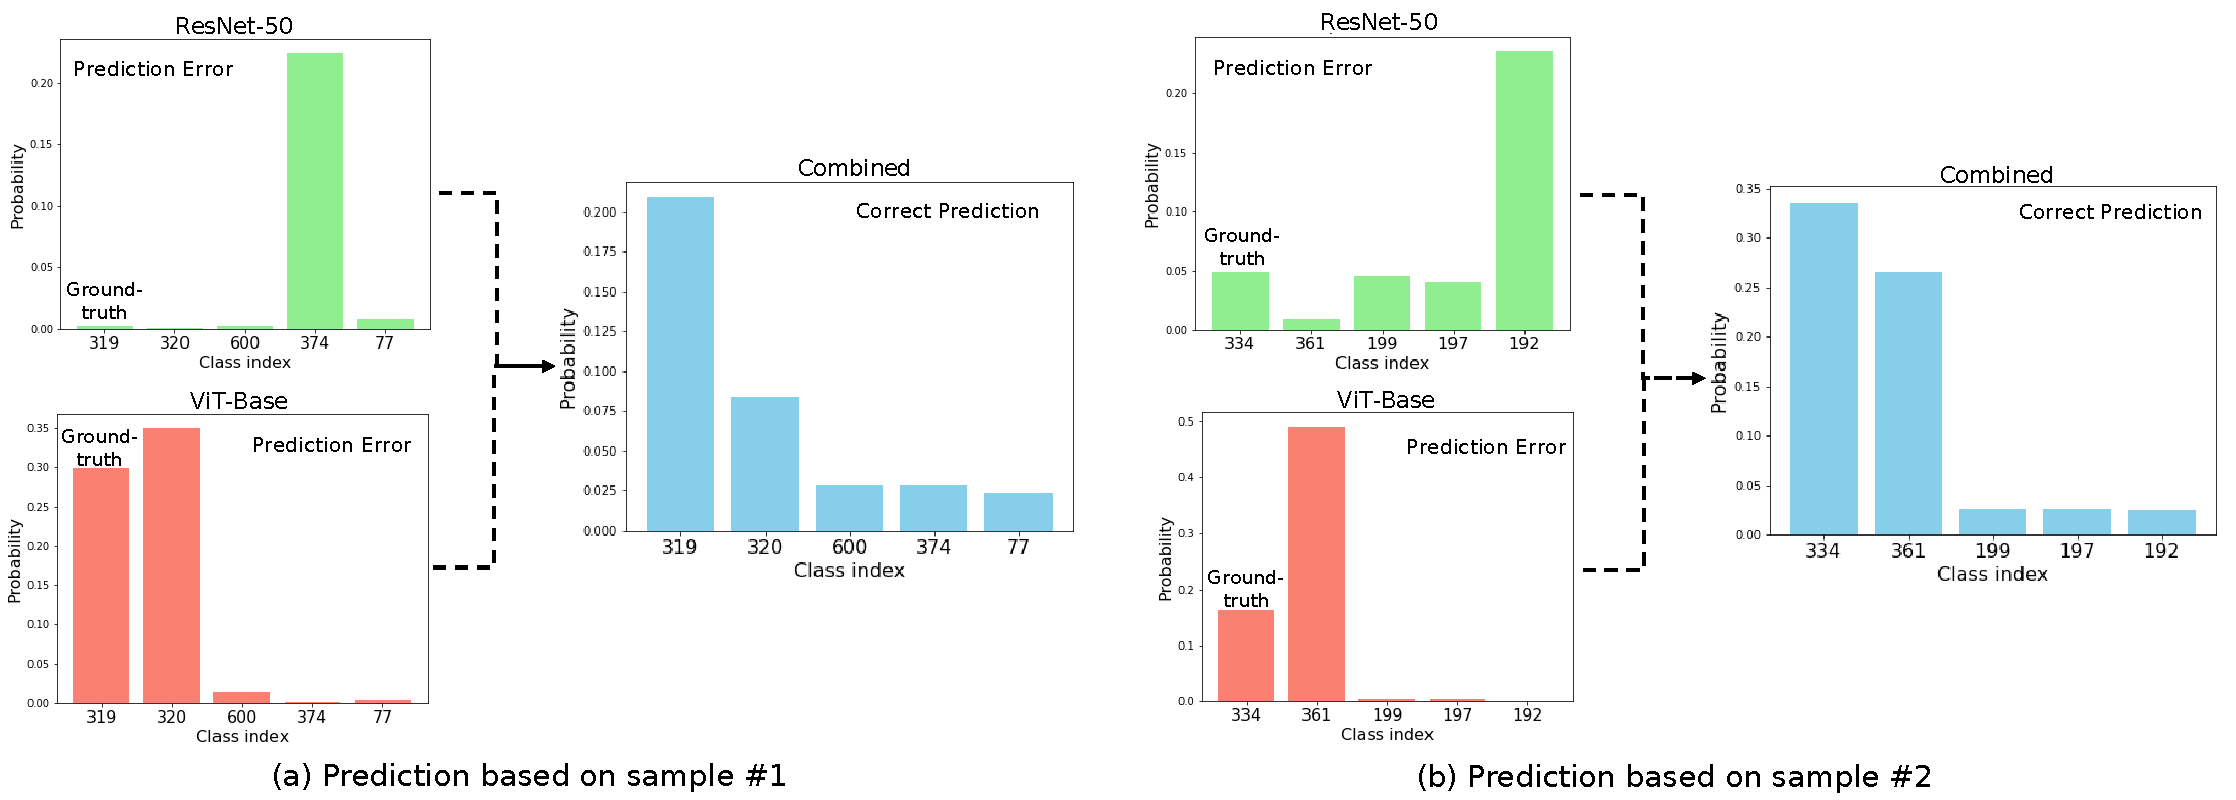
\includegraphics[width=0.93\linewidth]{sec/samplelevelvision.pdf}
    \vspace{-0.1in}
    \caption{A sample-level analysis highlights the advantages of our proposed cross-model co-learning approach. For each sample, we select the top five predicted probabilities from both ResNet-50 and ViT-Base. However, the final correct prediction, determined by COCA, differs from each of the initial predictions.}
    % A learnable parameter, $\tau$, is introduced to more effectively ensemble the outputs of the two models. The final predictions, $p_{com}(x)$, are derived from the combined outputs of both models.
    \vspace{-0.1in}
\label{samplelevel}
\end{figure*}


\section{Ratio Between Co-adaptation and Self-adaptation}
\label{Ratio}
COCA is designed to foster bidirectional improvement throughout the entire adaptation process. It can also be seamlessly integrated as a plug-and-play module to boost existing Test-Time Adaptation (TTA) methods. To keep our approach as simple as possible, we minimize the number of hyper-parameters, initially setting the co-adaptation to self-adaptation ratio to 1:1 as indicated in Eq.~\ref{fullloss}. Further experiments with \textit{EATA+COCA (ours)} on ImageNet-C reveal that a ratio of 1:2 slightly enhances accuracy—from 69.1\% to 69.5\%. Therefore, we view the 1:1 setting as a balanced compromise, offering faster computation with a modest performance trade-off compared to the marginal gains achieved with a higher computational cost.


\begin{table}[t]
\setlength{\tabcolsep}{11pt} % 调整列间距
    \renewcommand{\arraystretch}{0.9} % 增加行高
\resizebox{0.95\linewidth}{!}{%
\begin{tabular}{c|ccc|c}

\multicolumn{5}{c}{Sample \#1}\\ \midrule \midrule
Model \textbackslash Class & 98 & 146 & 356 & Predicted class \\ \midrule
ResNet-50 & 5.4 & 2.1 & 7.5 & 356 (\ding{55}) \\
ViT-Base & 5.9 & 8.6 & 1.6 & 146 (\ding{55}) \\
ResNet-50 / $\tau$ & 8.1 & 5.2 & 9.0 & - \\ \midrule
Combined & 7.0 & 6.9 & 5.3 & 98 (\checkmark)\\ \midrule 
\multicolumn{5}{c}{Sample \#2} \\ \midrule \midrule
Model\textbackslash Class & 192 & 334 & 361 & Predicted class \\ \midrule
ResNet-50 & 8.0 & 6.5 & 4.8 & 192 (\ding{55}) \\
ViT-Base & 1.6 & 6.9 & 8.0 & 361 (\ding{55}) \\
ResNet-50 / $\tau$ & 9.8 & 9.7 & 8.2 & - \\ \midrule
Combined & 5.7 & 8.3 & 8.1 & 334 (\checkmark)
\end{tabular}%
}
\vspace{-0.1in}
\caption{Further explanation of Fig.~\ref{samplelevel} on how COCA makes accurate predictions for these two samples. The values, all less than 10, represent the predicted logits. }
\label{Sampleleveltable}
\vspace{-0.2in}
\end{table}
% \


\section{The Influence of Model Weights}
\label{weights}
COCA remains effective even when the two models share the same deep architecture and differ only in their pre-trained weights. Table~\ref{samemodel} presents results based on ResNet-18 and ResNet-50, demonstrating that the cross-model co-learning mechanism remains robust. In this table, the superscript \textsuperscript{1} indicates that the model was pre-trained on the Instagram-1B hashtag dataset using semi-weakly supervised learning and fine-tuned on ImageNet~\cite{he2016deep}. Models without this superscript were initialized using the pre-trained weights provided by PyTorch. Notably, unlike previous findings, the performance of the anchor model does not consistently outperform that of the auxiliary model.



\begin{table}[t]
    % \vspace{-0.1in}
    \begin{center}
    \setlength{\tabcolsep}{9pt} % 调整列间距
    \renewcommand{\arraystretch}{1.1} % 增加行高
    \begin{threeparttable}
        \resizebox{\linewidth}{!}{
            \begin{tabular}{cc|ccc}
Anchor & Auxiliary & Anc. & Aux & \textbullet~Combined \\ \midrule
ResNet-18\textsuperscript{1} & ResNet-18 & 31.2 & 37.4 & 38.6 \\
ResNet-18 & ResNet-18\textsuperscript{1} & 37.2 & 31.0 & \textbf{39.9} \\ \midrule
ResNet-50\textsuperscript{1} & ResNet-50 & 41.7 & 45.8 & 48.5 \\
ResNet-50 & ResNet-50\textsuperscript{1} & 45.7 & 41.1 & \textbf{49.2}
\end{tabular}%
        }
    \end{threeparttable}
    \end{center}
    \vspace{-0.23in}
    \caption{Investigating whether COCA continues to deliver performance improvements when two models share the same deep architecture but differ in their pre-trained weights. Each result represents the average performance across 15 types of corruption on ImageNet-C (\%). For each pair, the two models have different pre-trained weights. }
    \label{samemodel}
    \vspace{-0.15in}
\end{table}



% section{Comparative Results on Cifar100-C dataset}
% \label{Cifar100-C}


\begin{table*}[t]
    \setlength{\tabcolsep}{3pt} % 调整列间距
    \renewcommand{\arraystretch}{1.1} % 增加行高
\resizebox{1.0\linewidth}{!}{%
\begin{tabular}{lccccccccccccccccc}
\multicolumn{1}{c}{} &  & \multicolumn{3}{c}{Noise} & \multicolumn{4}{c}{Blur} & \multicolumn{4}{c}{Weather} & \multicolumn{4}{c}{Digital} &  \\ \midrule
\multicolumn{1}{c|}{Methods} & \multicolumn{1}{c|}{Models} & Gauss & Shot & \multicolumn{1}{c|}{Impul} & Defoc & Glass & Motion & \multicolumn{1}{c|}{Zoom} & Snow & Frost & Fog & \multicolumn{1}{c|}{Brit} & Contr & Elastic & Pixel & \multicolumn{1}{c|}{JPEG} & Avg. \\ \midrule
\multicolumn{1}{l|}{\multirow{2}{*}{Source Only}} & \multicolumn{1}{c|}{ResNet-50} & 4.1 & 4.8 & \multicolumn{1}{c|}{2.0} & 26.1 & 11.2 & 26.1 & \multicolumn{1}{c|}{31.3} & 6.9 & 14.4 & 40.4 & \multicolumn{1}{c|}{9.6} & 36.9 & 20.1 & 11.5 & \multicolumn{1}{c|}{13.6} & 17.3 \\
\multicolumn{1}{l|}{} & \multicolumn{1}{c|}{ViT-Base} & 24.5 & 28.7 & \multicolumn{1}{c|}{29.4} & 59.6 & 23.3 & 53.1 & \multicolumn{1}{c|}{63.6} & 56.9 & 57.7 & 67.2 & \multicolumn{1}{c|}{70.6} & 76.2 & 45.3 & 36.2 & \multicolumn{1}{c|}{50.5} & 49.5 \\ \midrule
\multicolumn{1}{l|}{\multirow{2}{*}{Tent~\cite{wang2020tent}}} & \multicolumn{1}{c|}{ResNet-50} & 32.4 & 34.9 & \multicolumn{1}{c|}{33.2} & 64.9 & 38.7 & 61.0 & \multicolumn{1}{c|}{67.7} & 59.5 & 58.8 & 61.0 & \multicolumn{1}{c|}{73.3} & 67.0 & 51.8 & 59.7 & \multicolumn{1}{c|}{43.6} & 53.8 \\
\multicolumn{1}{l|}{} & \multicolumn{1}{c|}{ViT-Base} & 49.9 & 52.6 & \multicolumn{1}{c|}{56.1} & 76.5 & 32.5 & 71.5 & \multicolumn{1}{c|}{77.9} & 77.7 & 76.1 & 71.8 & \multicolumn{1}{c|}{88.9} & 74.3 & 58.5 & 42.8 & \multicolumn{1}{c|}{66.3} & 64.8 \\ \midrule
\multicolumn{1}{l|}{\multirow{2}{*}{EATA~\cite{niu2022efficient}}} & \multicolumn{1}{c|}{ResNet-50} & 35.5 & 37.4 & \multicolumn{1}{c|}{36.9} & 33.5 & 32.9 & 46.8 & \multicolumn{1}{c|}{52.5} & 51.6 & 45.8 & 60.0 & \multicolumn{1}{c|}{68.6} & 42.4 & 58.0 & 60.9 & \multicolumn{1}{c|}{55.5} & 55.4 \\
\multicolumn{1}{l|}{} & \multicolumn{1}{c|}{ViT-Base} & 54.1 & 54.8 & \multicolumn{1}{c|}{55.0} & 54.0 & 54.6 & 61.6 & \multicolumn{1}{c|}{57.8} & 63.5 & 62.8 & 71.3 & \multicolumn{1}{c|}{77.0} & 66.8 & 64.6 & 71.4 & \multicolumn{1}{c|}{68.1} & 66.7 \\ \midrule
\multicolumn{1}{l|}{\multirow{2}{*}{ROID~\cite{marsden2024universal2}}} & \multicolumn{1}{c|}{ResNet-50} & 36.2 & 39.5 & \multicolumn{1}{c|}{33.4} & 66.2 & 39.3 & 63.6 & \multicolumn{1}{c|}{68.0} & 62.5 & 62.2 & 64.8 & \multicolumn{1}{c|}{75.8} & 70.4 & 51.7 & 58.4 & \multicolumn{1}{c|}{42.4} & 55.6 \\
\multicolumn{1}{l|}{} & \multicolumn{1}{c|}{ViT-Base} & 55.6 & 57.9 & \multicolumn{1}{c|}{61.2} & 75.2 & 48.1 & 71.9 & \multicolumn{1}{c|}{77.1} & 73.3 & 75.5 & 76.4 & \multicolumn{1}{c|}{83.7} & 84.2 & 64.5 & 68.6 & \multicolumn{1}{c|}{64.4} & 69.2 \\ \midrule
\multicolumn{1}{l|}{\multirow{2}{*}{DeYO~\cite{lee2024entropy}}} & \multicolumn{1}{c|}{ResNet-50} & 35.9 & 39.4 & \multicolumn{1}{c|}{32.3} & 66.7 & 39.3 & 63.4 & \multicolumn{1}{c|}{68.1} & 62.4 & 61.7 & 65.1 & \multicolumn{1}{c|}{75.7} & 71.3 & 51.8 & 58.2 & \multicolumn{1}{c|}{42.2} & 55.6 \\
\multicolumn{1}{l|}{} & \multicolumn{1}{c|}{ViT-Base} & 49.6 & 52.7 & \multicolumn{1}{c|}{58.4} & 76.0 & 42.8 & 72.8 & \multicolumn{1}{c|}{76.7} & 73.9 & 74.3 & 75.9 & \multicolumn{1}{c|}{85.0} & 83.1 & 62.0 & 62.5 & \multicolumn{1}{c|}{62.6} & 67.2 \\ \midrule
\multicolumn{1}{l|}{\textbf{COCA\textsuperscript{1} (ours)}} & \multicolumn{1}{c|}{Combined} & 52.3 & 48.4 & \multicolumn{1}{c|}{65.6} & 81.2 & 55.1 & 79.5 & \multicolumn{1}{c|}{82.4} & 79.7 & 79.2 & 79.9 & \multicolumn{1}{c|}{88.2} & 87.2 & 69.1 & 77.1 & \multicolumn{1}{c|}{68.6} & 72.9 \\
\multicolumn{1}{l|}{\textbf{COCA\textsuperscript{2} (ours)}} & \multicolumn{1}{c|}{Combined} & \textbf{62.1} & \textbf{64.5} & \multicolumn{1}{c|}{\textbf{70.0}} & \textbf{82.4} & \textbf{61.8} & \textbf{80.1} & \multicolumn{1}{c|}{\textbf{82.3}} & \textbf{79.9} & \textbf{80.8} & \textbf{81.0} & \multicolumn{1}{c|}{\textbf{88.5}} & \textbf{87.5} & \textbf{71.9} & \textbf{77.6} & \multicolumn{1}{c|}{\textbf{69.4}} & \textbf{76.0}\\ \midrule
\end{tabular}
}
\vspace{-0.1in}
    \caption{Comparative results based on the Cifar100-C dataset (\%). COCA¹ and COCA² refer to the collaborations between ResNet-18 and ViT-Base, and between ResNet-50 and ViT-Base, respectively.}
    \label{cifar100c}
    % \vspace{-0.1in}

\end{table*}

\begin{table*}[t]
    \setlength{\tabcolsep}{8pt} % 调整列间距
    \renewcommand{\arraystretch}{1} % 增加行高
    
    \begin{center}
    \begin{threeparttable}
    \resizebox{1\linewidth}{!}{%
\begin{tabular}{c|ccccccccccc}
Model / Steps & $K=0$ & $K=1$ & $K=2$ & $K=3$ & $K=4$ & $K=5$ & $K=6$ & $K=7$ & $K=8$ & $K=9$ & $K=10$ \\ \midrule
ResNet-18 & 27.6 & 29.5 & 29.5 & 29.4 & 29.4 & 29.5 & 29.2 & 29.5 & 29.4 & 29.0 & 29.2 \\
ResNet-50* & 32.1 & 32.8 & 32.6 & 32.6 & 32.6 & 32.8 & 32.4 & 32.6 & 32.6 & 32.5 & 32.5 \\
\textbullet~Combined & 33.3 & 35.2 & 35.1 & 35.1 & 35.1 & 35.2 & 34.8 & 35.1 & 35.1 & 35.0 & 35.0 \\ \midrule
Mobile-ViT & 32.1 & 32.5 & 32.7 & 32.2 & 32.5 & 32.1 & 32.5 & 32.3 & 32.4 & 32.4 & 32.5 \\
ViT-Base* & 54.8 & 55.5 & 55.5 & 55.6 & 55.6 & 55.6 & 55.6 & 55.6 & 55.5 & 55.5 & 55.6 \\
\textbullet~Combined & 52.9 & 54.9 & 55.1 & 55.2 & 55.4 & 55.4 & 55.4 & 55.5 & 55.4 & 55.3 & 55.4 \\ \midrule
Mobile-ViT & 29.1 & 30.1 & 30.3 & 30.3 & 30.2 & 30.3 & 29.2 & 30.3 & 30.3 & 30.4 & 30.0 \\
ResNet-50* & 34.2 & 34.3 & 34.3 & 34.4 & 34.3 & 34.4 & 34.3 & 34.4 & 34.4 & 34.4 & 34.4 \\
\textbullet~Combined & 36.9 & 37.7 & 37.9 & 37.9 & 37.9 & 38.0 & 37.3 & 38.0 & 38.0 & 38.0 & 37.9 \\ \midrule
ResNet-50 & 40.9 & 41.8 & 41,5 & 41,5 & 41,5 & 41.5 & 41.6 & 41.6 & 41.6 & 41.6 & 41.6 \\
ViT-Base & 56.0 & 56.3 & 56.2 & 56.2 & 56.2 & 56.2 & 56.2 & 56.2 & 56.2 & 56.2 & 56.2 \\
\textbullet~Combined & 57.3 & 58.1 & 58.0 & 58.0 & 58.0 & 58.0 & 58.0 & 58.0 & 58.0 & 58.0 & 58.0\\ \midrule
\end{tabular}%
 }

    \end{threeparttable}
    \end{center}
    \vspace{-0.2in}
    \caption{Impact of the parameter update iterations, $K$, for $\tau$ on cross-model collaborative learning performance (\%). An asterisk (*) denotes the anchor model. This experiment is also based on ImageNet-C (Gaussian Noise under severity level 5). $K=0$ represents that the outputs of two pre-trained models are combined by averaging, without learning $\tau$. }
    \label{tepoch}
    \vspace{-0.1in}
\end{table*}









% \section{Comparative Results on ImageNet-R and ImageNet-Sketch dataset}
% \label{ImageNetMore}




\section{More Analysis on the Influence of Model Parameters and Architectures}
\label{MoreAcross}

Two key insights emerge from the extensive comparative results: 1) More parameters enhance performance. Increasing the parameter count in the auxiliary model enhances overall performance when the anchor model is fixed. For instance, the accuracy improves from 64.9\% with ResNet-50 and ViT-Base to 67.1\% with ResNet-101 and ViT-Base. This improvement is likely because models with more parameters and the same deep architecture can facilitate more comprehensive learning. 2) Architectural diversity offers benefits. Diversity in deep architectures between models improves performance. For pairs of models sharing one common model, the pair with differing architectures outperforms the one with similar parameter sizes but identical architectures. For example, the accuracy of ResNet-18 and ResNet-50 is 45.6\%, while Mobile-ViT and ResNet-50 achieve 50.5\%. This advantage may arise because distinct architectures enable the models to learn more diverse representations from the same source domain.




% \section{More Results Across Different Model Pairs}
% \label{allmodelsappendix}

% In Section~\ref{sec:Experimental Section} of the main paper, we discuss the generalizability of COCA-based model collaboration and only report 6 results of all models pair-wise collaboration. Additionally, in the appendix to this chapter, we present further experimental results. Specifically, we selected six models to collaborate with one another. Following the anchor model selection strategy mentioned in Section~\ref{tintro}, we conducted total 15 experiment results on model collaboration, the results of which are summarized in the table in the Table.~\ref{allmodelssup1} and~\ref{allmodelssup2}.

% In Section~\ref{sec:Experimental Section} of the main paper, we discussed the impact of model architecture on co-learning, using six different deep architectures. Due to page limitations, additional results are provided in Table~\ref{allmodelssup1} of the Supplementary Material. As demonstrated in this table, co-learning between two models significantly outperforms the individual adaptation of each model, which relies solely on the complementary knowledge from the other model.

% In Section~\ref{sec:Experimental Section} of the main paper, we employed six different deep architectures to investigate the impact of model design on our proposed approach, COCA (cross-model co-learning TTA). Due to space limitations, additional results are provided in Table~\ref{allmodelssup}  of the Supplementary Material. From these tables, we can draw two key conclusions. First, COCA consistently delivers strong performance across different pairs of deep architectures, although its performance varies depending on the specific model pair. Second, under COCA, each model consistently outperforms single-model adaptation using self-supervised knowledge \cite{wang2020tent}, as shown in Table~\ref{params} of the main paper.





% \begin{table*}[t]
% \vspace{-0.2in}
%     \setlength{\tabcolsep}{3pt} % 调整列间距
%     \renewcommand{\arraystretch}{1.05} % 增加行高
%     \begin{center}
%     \begin{threeparttable}
%     \resizebox{0.9\linewidth}{!}{%
%     \begin{tabular}{c|ccc|cccc|cccc|cccc|c}
%  \multicolumn{1}{c}{}& \multicolumn{3}{c}{Noise} & \multicolumn{4}{c}{Blur} & \multicolumn{4}{c}{Weather} & \multicolumn{4}{c}{Digital} &  \\ \midrule
% Models & Gauss & Shot & Impul & Defoc & Glass & Motion & Zoom & Snow & Frost & Fog & Brit & Contr & Elastic & Pixel & JPEG & Avg. \\ \midrule
%  \midrule
% \end{tabular}%
%         }
%     \end{threeparttable}
%     \end{center}
%     \vspace{-0.25in}
%     \caption{Additional experimental results for different pairs of networks (\%) on ImageNet-C (severity level 5) are provided. An asterisk (*) denotes the anchor model.}
%     \label{allmodelssup1}
%     \vspace{-0.2in}
% \end{table*}



% \begin{table*}[t]
    
%     \setlength{\tabcolsep}{3pt} % 调整列间距
%     \renewcommand{\arraystretch}{1.0} % 增加行高
    
%     \begin{center}
%     \begin{threeparttable}
%         \resizebox{1.0\linewidth}{!}{%
%             \begin{tabular}{c|ccc|cccc|cccc|cccc|c}
%                 \multicolumn{1}{c}{} & \multicolumn{3}{c}{Noise} & \multicolumn{4}{c}{Blur} & \multicolumn{4}{c}{Weather} & \multicolumn{4}{c}{Digital} &  \\
%                 \midrule
%                 Models & Gauss & Shot & Impul & Defoc & Glass & Motion & Zoom & Snow & Frost & Fog & Brit & Contr & Elastic & Pixel & JPEG & Avg. \\ 
%                 \midrule
%                 Mobile-ViT & 29.7 & 29.0 & 33.2 & 30.1 & 26.5 & 44.8 & 50.9 & 51.3 & 48.0 & 60.8 & 70.0 & 41.9 & 54.0 & 54.6 & 52.1 & 45.1 \\
%                 ResNet-50* & 34.0 & 35.9 & 35.7 & 32.3 & 31.5 & 45.9 & 51.1 & 50.4 & 43.8 & 59.1 & 67.9 & 41.0 & 56.5 & 59.8 & 54.4 & 46.6 \\
%                 \textbullet~Combined & \textbf{37.2} & \textbf{38.1} & \textbf{39.8} & \textbf{35.9} & \textbf{33.7} & \textbf{50.2} & \textbf{55.3} & \textbf{55.6} & \textbf{50.1} & \textbf{63.8} & \textbf{72.3} & \textbf{45.9} & \textbf{59.6} & \textbf{62.1} & \textbf{58.0} & \textbf{50.5} \\
%                 \midrule
%                 ResNet-50 & 34.6 & 37.6 & 36.7 & 32.9 & 32.7 & 47.9 & 52.5 & 51.4 & 41.1 & 59.8 & 67.4 & 22.6 & 57.9 & 60.8 & 55.7 & 46.1 \\
%                 ResNet-101* & 36.0 & 39.2 & 38.2 & 34.8 & 35.4 & 49.3 & 55.1 & 53.2 & 43.1 & 61.3 & 69.6 & 24.5 & 60.3 & 62.5 & 57.7 & 48.0 \\
%                 \textbullet~Combined & \textbf{38.7} & \textbf{41.9} & \textbf{41.0} & \textbf{36.8} & \textbf{37.0} & \textbf{52.4} & \textbf{57.3} & \textbf{55.8} & \textbf{45.1} & \textbf{63.7} & \textbf{71.3} & \textbf{25.6} & \textbf{62.5} & \textbf{65.0} & \textbf{60.1} & \textbf{50.3} \\
%                 \midrule
%                 Mobile-ViT & 32.6 & 34.7 & 35.8 & 33.1 & 32.2 & 46.9 & 50.4 & 54.0 & 51.4 & 61.4 & 70.7 & 46.5 & 55.0 & 55.0 & 53.4 & 47.5 \\
%                 ViT-Base* & \textbf{55.6} & 55.9 & 56.9 & 57.2 & \textbf{55.7} & 62.6 & 58.8 & 65.5 & 64.5 & 73.0 & 78.2 & \textbf{69.8} & 65.6 & 71.2 & 68.7 & 64.0 \\
%                 \textbullet~Combined & 55.2 & \textbf{56.0} & \textbf{57.1} & \textbf{57.3} & 55.6 & \textbf{63.5} & \textbf{61.1} & \textbf{67.3} & \textbf{65.5} & \textbf{73.7} & \textbf{78.8} & 69.0 & \textbf{67.5} & \textbf{71.3} & \textbf{68.8} & \textbf{64.5} \\
%                 \midrule
%                 Mobile-ViT & 31.6 & 34.8 & 35.3 & 32.1 & 32.0 & 47.2 & 51.9 & 53.4 & 50.8 & 61.6 & 70.3 & 45.7 & 55.1 & 55.6 & 53.1 & 47.4 \\
%                 ViT-Large* & 66.0 & 67.4 & 68.2 & 63.6 & 63.4 & 70.4 & 67.9 & 75.8 & 71.6 & 77.4 & \textbf{83.7} & 75.7 & 71.4 & 77.3 & \textbf{75.6} & 71.7 \\
%                 \textbullet~Combined & \textbf{66.4} & \textbf{67.8} & \textbf{68.6} & \textbf{64.0} & \textbf{63.8} & \textbf{70.4} & \textbf{69.0} & \textbf{76.2} & \textbf{72.4} & \textbf{77.8} & 83.4 & \textbf{76.1} & \textbf{72.8} & \textbf{76.8} & 75.2 & \textbf{72.0} \\
%                 \midrule
%                 ResNet-50 & 42.5 & 44.5 & 43.5 & 41.0 & 40.5 & 52.2 & 54.4 & 55.0 & 49.7 & 61.6 & 68.5 & 51.8 & 59.8 & 62.7 & 57.6 & 52.3 \\
%                 ViT-Large* & 66.3 & 67.7 & 68.7 & 63.8 & 64.1 & 70.9 & 68.5 & 76.0 & 71.7 & 77.5 & 83.8 & 76.1 & 71.6 & 77.8 & 75.9 & 72.0 \\
%                 \textbullet~Combined & \textbf{67.1} & \textbf{68.5} & \textbf{69.3} & \textbf{64.8} & \textbf{64.9} & \textbf{71.9} & \textbf{70.2} & \textbf{76.7} & \textbf{72.3} & \textbf{78.2} & \textbf{83.9} & \textbf{76.4} & \textbf{73.6} & \textbf{78.6} & \textbf{76.7} & \textbf{72.9} \\
%                 \midrule
%                 ViT-Base & 58.2 & 58.7 & 59.2 & 59.9 & 58.9 & 64.4 & 60.5 & 66.4 & 64.5 & 73.7 & 78.6 & 71.5 & 66.4 & 72.6 & 70.1 & 65.6 \\
%                 ViT-Large* & 66.4 & 67.5 & 68.4 & 63.8 & 63.8 & 70.5 & 66.6 & 74.3 & 71.6 & 77.1 & 83.7 & 76.1 & 70.3 & 77.4 & 75.6 & 71.5 \\
%                 \textbullet~Combined & \textbf{67.7} & \textbf{68.8} & \textbf{69.4} & \textbf{65.9} & \textbf{65.5} & \textbf{71.7} & \textbf{67.8} & \textbf{74.8} & \textbf{72.4} & \textbf{78.5} & \textbf{83.8} & \textbf{77.3} & \textbf{72.3} & \textbf{78.3} & \textbf{76.1} & \textbf{72.7} \\
%                 \midrule
%             \end{tabular}%
%         }
%     \end{threeparttable}
%     \end{center}
%     \vspace{-0.2in}
%     \caption{The performance of COCA across different model pairs, with results on ImageNet-C (\%). Additional results can be found in Appendix~\ref{allmodelsappendix}.}
%     \label{allmodels}
%     \vspace{-0.1in}
% \end{table*}






\begin{table*}[t]
    \setlength{\tabcolsep}{3pt} % 调整列间距
    \renewcommand{\arraystretch}{1.03} % 增加行高
    \begin{center}
    \begin{threeparttable}
        \resizebox{0.95\linewidth}{!}{%
    \begin{tabular}{c|ccc|cccc|cccc|cccc|c}
 \multicolumn{1}{c}{}& \multicolumn{3}{c}{Noise} & \multicolumn{4}{c}{Blur} & \multicolumn{4}{c}{Weather} & \multicolumn{4}{c}{Digital} &  \\ \midrule
Models & Gauss & Shot & Impul & Defoc & Glass & Motion & Zoom & Snow & Frost & Fog & Brit & Contr & Elastic & Pixel & JPEG & Avg. \\ \midrule
Mobile-ViT & 29.6 & 32.5 & 32.9 & 30.2 & 29.3 & 44.5 & 50.7 & 52.0 & 47.7 & 60.4 & 70.1 & 41.9 & 54.1 & 54.7 & 52.3 & { 45.5} \\
ResNet-18* & 28.5 & 30.3 & 29.0 & 26.6 & 26.8 & 37.6 & 43.8 & 41.9 & 37.3 & 51.2 & 60.2 & 34.2 & 49.3 & 52.5 & 48.1 & { 39.8} \\
\textbullet~Combined & \textbf{34.9} & \textbf{37.3} & \textbf{36.7} & \textbf{33.8} & \textbf{33.0} & \textbf{47.6} & \textbf{53.3} & \textbf{53.7} & \textbf{48.7} & \textbf{61.7} & \textbf{70.4} & \textbf{43.9} & \textbf{57.6} & \textbf{59.2} & \textbf{56.0} & { \textbf{48.5}} \\ \midrule
Mobile-ViT & 29.7 & 29.0 & 33.2 & 30.1 & 26.5 & 44.8 & 50.9 & 51.3 & 48.0 & 60.8 & 70.0 & 41.9 & 54.0 & 54.6 & 52.1 & { 45.1} \\
ResNet-50* & 34.0 & 35.9 & 35.7 & 32.3 & 31.5 & 45.9 & 51.1 & 50.4 & 43.8 & 59.1 & 67.9 & 41.0 & 56.5 & 59.8 & 54.4 & { 46.6} \\
\textbullet~Combined & \textbf{37.2} & \textbf{38.1} & \textbf{39.8} & \textbf{35.9} & \textbf{33.7} & \textbf{50.2} & \textbf{55.3} & \textbf{55.6} & \textbf{50.1} & \textbf{63.8} & \textbf{72.3} & \textbf{45.9} & \textbf{59.6} & \textbf{62.1} & \textbf{58.0} & { \textbf{50.5}} \\ \midrule
Mobile-ViT & 30.9 & 33.5 & 33.5 & 31.8 & 30.5 & 46.2 & 51.5 & 53.3 & 50.1 & 61.1 & 69.6 & 44.8 & 55.0 & 55.2 & 53.0 & { 46.7} \\
ResNet-101* & 37.7 & 39.8 & 38.9 & 36.8 & 36.8 & 49.8 & 54.8 & 54.3 & 49.0 & 61.7 & 69.5 & 47.9 & 60.0 & 62.3 & 57.5 & { 50.5} \\
\textbullet~Combined & \textbf{39.9} & \textbf{42.3} & \textbf{42.0} & \textbf{39.2} & \textbf{38.6} & \textbf{53.4} & \textbf{57.9} & \textbf{59.1} & \textbf{54.8} & \textbf{66.0} & \textbf{73.2} & \textbf{52.1} & \textbf{62.4} & \textbf{63.8} & \textbf{60.1} & { \textbf{53.7}} \\ \midrule
ResNet-50 & 34.6 & 37.6 & 36.7 & 32.9 & 32.7 & 47.9 & 52.5 & 51.4 & 41.1 & 59.8 & 67.4 & 22.6 & 57.9 & 60.8 & 55.7 & 46.1 \\
ResNet-101* & 36.0 & 39.2 & 38.2 & 34.8 & 35.4 & 49.3 & 55.1 & 53.2 & 43.1 & 61.3 & 69.6 & 24.5 & 60.3 & 62.5 & 57.7 & 48.0 \\
\textbullet~Combined & \textbf{38.7} & \textbf{41.9} & \textbf{41.0} & \textbf{36.8} & \textbf{37.0} & \textbf{52.4} & \textbf{57.3} & \textbf{55.8} & \textbf{45.1} & \textbf{63.7} & \textbf{71.3} & \textbf{25.6} & \textbf{62.5} & \textbf{65.0} & \textbf{60.1} & \textbf{50.3} \\ \midrule
Mobile-ViT & 32.6 & 34.7 & 35.8 & 33.1 & 32.2 & 46.9 & 50.4 & 54.0 & 51.4 & 61.4 & 70.7 & 46.5 & 55.0 & 55.0 & 53.4 & 47.5 \\
ViT-Base* & \textbf{55.6} & 55.9 & 56.9 & 57.2 & \textbf{55.7} & 62.6 & 58.8 & 65.5 & 64.5 & 73.0 & 78.2 & \textbf{69.8} & 65.6 & 71.2 & 68.7 & 64.0 \\
\textbullet~Combined & 55.2 & \textbf{56.0} & \textbf{57.1} & \textbf{57.3} & 55.6 & \textbf{63.5} & \textbf{61.1} & \textbf{67.3} & \textbf{65.5} & \textbf{73.7} & \textbf{78.8} & 69.0 & \textbf{67.5} & \textbf{71.3} & \textbf{68.8} & \textbf{64.5} \\ \midrule
Mobile-ViT & 31.6 & 34.8 & 35.3 & 32.1 & 32.0 & 47.2 & 51.9 & 53.4 & 50.8 & 61.6 & 70.3 & 45.7 & 55.1 & 55.6 & 53.1 & 47.4 \\
ViT-Large* & 66.0 & 67.4 & 68.2 & 63.6 & 63.4 & 70.4 & 67.9 & 75.8 & 71.6 & 77.4 & \textbf{83.7} & 75.7 & 71.4 & 77.3 & \textbf{75.6} & 71.7 \\
\textbullet~Combined & \textbf{66.4} & \textbf{67.8} & \textbf{68.6} & \textbf{64.0} & \textbf{63.8} & \textbf{70.4} & \textbf{69.0} & \textbf{76.2} & \textbf{72.4} & \textbf{77.8} & 83.4 & \textbf{76.1} & \textbf{72.8} & \textbf{76.8} & 75.2 & \textbf{72.0} \\ \midrule
ResNet-50 & 42.5 & 44.5 & 43.5 & 41.0 & 40.5 & 52.2 & 54.4 & 55.0 & 49.7 & 61.6 & 68.5 & 51.8 & 59.8 & 62.7 & 57.6 & 52.3 \\
ViT-Large* & 66.3 & 67.7 & 68.7 & 63.8 & 64.1 & 70.9 & 68.5 & 76.0 & 71.7 & 77.5 & 83.8 & 76.1 & 71.6 & 77.8 & 75.9 & 72.0 \\
\textbullet~Combined & \textbf{67.1} & \textbf{68.5} & \textbf{69.3} & \textbf{64.8} & \textbf{64.9} & \textbf{71.9} & \textbf{70.2} & \textbf{76.7} & \textbf{72.3} & \textbf{78.2} & \textbf{83.9} & \textbf{76.4} & \textbf{73.6} & \textbf{78.6} & \textbf{76.7} & \textbf{72.9} \\ \midrule
ViT-Base & 58.2 & 58.7 & 59.2 & 59.9 & 58.9 & 64.4 & 60.5 & 66.4 & 64.5 & 73.7 & 78.6 & 71.5 & 66.4 & 72.6 & 70.1 & 65.6 \\
ViT-Large* & 66.4 & 67.5 & 68.4 & 63.8 & 63.8 & 70.5 & 66.6 & 74.3 & 71.6 & 77.1 & 83.7 & 76.1 & 70.3 & 77.4 & 75.6 & 71.5 \\
\textbullet~Combined & \textbf{67.7} & \textbf{68.8} & \textbf{69.4} & \textbf{65.9} & \textbf{65.5} & \textbf{71.7} & \textbf{67.8} & \textbf{74.8} & \textbf{72.4} & \textbf{78.5} & \textbf{83.8} & \textbf{77.3} & \textbf{72.3} & \textbf{78.3} & \textbf{76.1} & \textbf{72.7} \\ \midrule
ResNet-18 & 29.0 & 30.9 & 30.3 & 25.4 & 26.3 & 39.1 & 44.7 & 43.2 & 32.9 & 52.2 & 60.2 & 16.3 & 50.5 & 53.5 & 49.1 & { 38.9} \\
ResNet50* & 32.4 & 34.7 & 34.4 & 29.2 & 29.6 & 44.8 & 51.1 & 49.6 & 38.3 & 58.7 & 67.6 & 19.3 & 56.7 & 59.8 & 54.3 & { 44.0} \\
\textbullet~Combined & \textbf{34.8} & \textbf{37.1} & \textbf{36.6} & \textbf{31.0} & \textbf{31.5} & \textbf{46.8} & \textbf{52.4} & \textbf{51.3} & \textbf{39.6} & \textbf{60.0} & \textbf{68.0} & \textbf{20.1} & \textbf{58.1} & \textbf{61.0} & \textbf{56.1} & { \textbf{45.6}} \\ \midrule
ResNet-50 & 41.6 & 43.2 & 43.2 & 40.6 & 39.5 & 51.4 & 48.5 & 50.7 & 42.3 & 61.5 & 68.4 & 51.5 & 58.5 & 62.4 & 57.2 & 50.7 \\
ViT-Base & 56.4 & 56.7 & 57.6 & 58.2 & 56.5 & 62.7 & 55.9 & 61.9 & 53.6 & 73.2 & 78.1 & 70.1 & 66.0 & 72.0 & 69.0 & 63.2 \\
\textbullet~Combined & \textbf{58.3} & \textbf{58.8} & \textbf{59.6} & \textbf{59.5} & \textbf{57.9} & \textbf{64.9} & \textbf{58.4} & \textbf{63.9} & \textbf{54.9} & \textbf{74.3} & \textbf{78.8} & \textbf{70.8} & \textbf{68.9} & \textbf{73.6} & \textbf{70.6} & \textbf{64.9} \\ \midrule
ResNet-18 & 30.7 & 33.5 & 30.8 & 27.9 & 27.4 & 40.0 & 45.3 & 43.8 & 34.0 & 52.4 & 60.3 & 20.1 & 50.9 & 53.6 & 49.4 & { 40.0} \\
ResNet-101* & 36.4 & 39.3 & 37.1 & 34.4 & 33.9 & 48.7 & 54.5 & 52.6 & 41.8 & 61.0 & 69.3 & 24.8 & 60.2 & 62.4 & 57.8 & { 47.6} \\
\textbullet~Combined & \textbf{38.7} & \textbf{41.4} & \textbf{39.1} & \textbf{35.9} & \textbf{35.2} & \textbf{50.1} & \textbf{55.6} & \textbf{53.8} & \textbf{42.9} & \textbf{62.1} & \textbf{69.8} & \textbf{25.8} & \textbf{61.2} & \textbf{63.5} & \textbf{58.9} & { \textbf{48.9}} \\ \midrule
ResNet-18 & 34.3 & 36.2 & 34.8 & 32.8 & 32.6 & 41.9 & 43.7 & 42.7 & 37.3 & 53.4 & 60.7 & 42.3 & 51.0 & 54.5 & 50.3 & { 43.2} \\
{ ViT-Base*} & 55.8 & 56.1 & 57.0 & 57.7 & 56.2 & 62.2 & 57.5 & 62.0 & 57.6 & 72.9 & 77.9 & 69.8 & 65.3 & 71.7 & 68.7 & { 63.2} \\
\textbullet~Combined & \textbf{56.8} & \textbf{57.5} & \textbf{58.1} & \textbf{58.7} & \textbf{57.1} & \textbf{63.6} & \textbf{59.4} & \textbf{63.4} & \textbf{58.2} & \textbf{73.6} & \textbf{77.9} & \textbf{70.1} & \textbf{67.3} & \textbf{72.6} & \textbf{69.6} & { \textbf{64.3}} \\ \midrule
ResNet-18 & 34.8 & 36.7 & 34.8 & 33.0 & 33.1 & 42.4 & 46.2 & 45.8 & 41.0 & 53.2 & 60.9 & 42.2 & 51.5 & 54.6 & 50.6 & { 44.1} \\
ViT-Large* & 66.3 & 67.6 & 68.4 & 63.6 & 63.5 & 70.8 & 67.9 & 76.0 & 71.7 & 77.3 & 83.9 & 76.0 & 71.5 & 77.8 & 75.8 & { 71.9} \\
\textbullet~Combined & \textbf{66.8} & \textbf{68.1} & \textbf{68.9} & \textbf{64.2} & \textbf{64.1} & \textbf{71.3} & \textbf{69.0} & \textbf{76.1} & \textbf{72.0} & \textbf{77.8} & \textbf{83.8} & \textbf{75.9} & \textbf{72.8} & \textbf{78.3} & \textbf{76.2} & { \textbf{72.3}} \\ \midrule
ResNet-101 & 42.2 & 43.8 & 43.6 & 41.8 & 41.7 & 50.3 & 52.8 & 53.7 & 49.3 & 59.6 & 65.7 & 49.8 & 57.6 & 59.8 & 56.3 & \multicolumn{1}{l}{51.2} \\
ViT-Base* & 57.2 & 58.2 & 58.5 & 59.2 & 58.3 & 64.2 & 61.6 & 67.7 & 66.7 & 74.0 & 79.1 & 70.6 & 68.1 & 73.1 & 70.7 & \multicolumn{1}{l}{65.8} \\
\textbullet~Combined & \textbf{58.7} & \textbf{60.2} & \textbf{60.1} & \textbf{60.5} & \textbf{59.5} & \textbf{66.1} & \textbf{64.2} & \textbf{69.4} & \textbf{67.5} & \textbf{74.8} & \textbf{79.0} & \textbf{70.9} & \textbf{70.3} & \textbf{74.3} & \textbf{71.7} & \multicolumn{1}{l}{\textbf{67.1}}\\ \midrule


ResNet-101 & 46.1 & 48.1 & 47.4 & 45.2 & 45.5 & 56.1 & 57.9 & 58.8 & 53.2 & 64.1 & 70.3 & 55.0 & 62.7 & 65.1 & 60.6 & { 55.7} \\
ViT-Large* & 66.3 & 67.8 & 68.6 & 63.8 & 64.2 & 71.0 & 68.3 & 76.1 & 71.7 & 77.4 & 83.9 & 76.0 & 71.7 & 77.9 & 76.0 & { 72.1} \\
\textbullet~Combined & \textbf{67.3} & \textbf{68.8} & \textbf{69.3} & \textbf{65.0} & \textbf{65.4} & \textbf{72.2} & \textbf{70.3} & \textbf{76.8} & \textbf{72.4} & \textbf{78.4} & \textbf{84.0} & \textbf{76.4} & \textbf{74.3} & \textbf{78.7} & \textbf{76.8} & { \textbf{73.1}} \\ \midrule

\end{tabular}%
        }
    \end{threeparttable}
    \end{center}
    \vspace{-0.2in}
    \caption{Comparison of accuracy (\%) on ImageNet-C (level 5) with pairwise collaboration of all models. An asterisk (*) denotes the anchor model.}
    \label{allmodelssup}
    % \vspace{-0.1in}
\end{table*}


% \STATE Compute marginal entropy loss $\mathcal{L}_{mar}(p_{e}(\bx))$ \COMMENT{Eq.~\ref{marginalent}}
%         \STATE Compute cross-model knowledge distillation loss $\mathcal{L}_{ckd}(p_{1}(\bx), p_{2}(\bx), \hat{y})$ 

% 
% Having the supplementary compiled together with the main paper means that:



\section{The Applicability of COCA to More Than Two Models}\label{suppl:sec:three-models}
The general procedure follows a similar structure to the pseudocode outlined in Algorithm 1. Given three models, denoted as M1, M2, and M3, we rank them by size in descending order: M1 $>$ M2 $>$ M3. The co-learning process is conducted in two steps: 1) M2 and M3 are designated as the anchor model and auxiliary model, respectively. COCA is trained using these two models. 2) M1 and the combination of M2 and M3 are designated as the anchor model and auxiliary model, respectively. COCA is then re-trained using this setup to produce the final performance results. The results of this process are summarized in Table~\ref{multimodles}, demonstrating an improvement in average performance across all conditions, highlighting COCA’s effectiveness across three models.  

% However, for the \textit{Contr} domain, introducing a third model leads to a decrease in COCA's performance. Similarly, the findings in Table~\ref{allmodelssup} also indicate that COCA's performance becomes harder to improve when a smaller model is introduced as the auxiliary model. The reason for this could be that knowledge extraction is inherently easier in this type of domain.

We further investigate the applicability of COCA by incorporating a third small model to collaborate with a pair of small models. To diversify the model selection, we include PiT~\cite{heo2021rethinking}, a pooling-based Vision Transformer, which differs from both ViT and ResNet. PiT has 10.6M parameters and achieves 31.8\% accuracy (averaged across 15 corruptions in ImageNet-C) with Tent~\cite{wang2020tent}. As shown in Table~\ref{multimodles}, incorporating a third model further enhances the overall performance.


\vfill
% In our Coca, we mainly focus on the mutual collaboration of models, so we have designed an anchor model dominated collaboration mechanism for the mutual collaboration between two models. So, when expanding to more models, how should the anchor collaboration mechanism based on the two models be applied? We have designed an additive anchoring collaboration mechanism for this purpose, which breaks down the collaboration problem of multiple models into an iterative collaboration problem of two models. Specifically, we first select two models with larger parameter quantities as the basis, apply two models anchor collaboration mechanisms on these two models, and then select the remaining models with larger parameter quantities as the collaborative combination with the previous models to apply anchor collaboration mechanisms. From the results shown in Table~\ref{multimodles}, We can draw the following two conclusions: (1) As the number of models added increases, in most cases, it can bring performance improvement, which demonstrates the effectiveness of the COCA model collaboration mechanism. (2) In the collaboration of multiple models, the structure and parameter quantity of the models mentioned in Chapter 3 of the main text still have an impact on the rules of model collaboration.

% \afterpage{
    \clearpage

\begin{table*}[t]
    % \vspace{-0.3in}
    \setlength{\tabcolsep}{3pt} % 调整列间距
    \renewcommand{\arraystretch}{1.2} % 增加行高
    \begin{center}
    \begin{threeparttable}
        \resizebox{\linewidth}{!}{%
    \begin{tabular}{c|ccc|cccc|cccc|cccc|c}
 \multicolumn{1}{c}{}& \multicolumn{3}{c}{Noise} & \multicolumn{4}{c}{Blur} & \multicolumn{4}{c}{Weather} & \multicolumn{4}{c}{Digital} &  \\ \midrule
Models & Gauss. & Shot & Impul. & Defoc. & Glass & Motion & Zoom & Snow & Frost & Fog & Brit. & Contr. & Elastic & Pixel & JPEG & Avg. \\ \midrule
RN-50 + ViT-B* & 58.3 & 58.8 & 59.6 & 59.5 & 57.9 & 64.9 & 58.4 & 63.9 & 54.9 & 74.3 & 78.8 & 70.8 & 68.9 & 73.6 & 70.6 & 64.9 \\ \midrule 
\textcolor{blue}{RN-18} + RN-50 + ViT-B* & 58.8 & 59.8 & 60.2 & 59.2 & 59.0 & 66.3 & 65.7 & 69.5 & 61.0 & 75.1 & 78.5 & 69.5 & 71.3 & 74.4 & 71.8 & 66.7 \\ \midrule \midrule
RN-101 + ViT-B* & 58.8 & 59.3 & 59.7 & 59.7 & 58.9 & 65.6 & 59.7 & 63.9 & 55.0 & 74.4 & 79.0 & 71.3 & 69.7 & 74.0 & 71.1 & 65.3 \\ \midrule 
\textcolor{blue}{RN-50} + RN-101 + ViT-B* & 59.7 & 60.9 & 61.0 & 60.0 & 60.1 & 67.8 & 67.0 & 70.6 & 60.0 & 75.6 & 79.2 & 70.4 & 72.5 & 75.0 & 72.5 & 67.5 \\ \midrule
\textcolor{blue}{M-ViT} + RN-101 + ViT-B* & 56.7 & 57.7 & 58.2 & 57.7 & 57.2 & 65.6 & 65.0 & 69.9 & 61.3 & 74.5 & 79.0 & 68.5 & 70.9 & 73.3 & 70.4 & 65.7 \\ \midrule \midrule
ViT-B + ViT-L* & 67.7 & 68.8 & 69.4 & 65.9 & 65.5 & 71.7 & 67.8 & 74.8 & 72.4 & 78.5 & 83.8 & 77.3 & 72.3 & 78.3 & 76.1 & 72.7 \\ \midrule 
\textcolor{blue}{M-ViT} + ViT-B + ViT-L* & 68.7 & 70.1 & 70.7 & 67.3 & 67.5 & 71.2 & 70.0 & 75.5 & 73.0 & 78.8 & 83.0 & 77.7 & 74.8 & 77.8 & 75.5 & 73.4 \\ \midrule
\textcolor{blue}{RN-101} + ViT-B + ViT-L* & 68.8 & 69.8 & 70.4 & 67.2 & 67.8 & 73.4 & 72.0 & 77.3 & 62.3 & 79.9 & 83.8 & 77.2 & 76.8 & 80.0 & 77.6 & 73.6 \\ \midrule \midrule
RN-34 + M-ViT* & 24.2 & 27.5 & 25.3 & 25.7 & 29.7 & 41.8 & 50.9 & 49.7 & 48.3 & 59.0 & 71.1 & 36.6 & 52.7 & 52.0 & 49.3 & 43.0 \\ \midrule 
\textcolor{blue}{RN-18} + RN-34 + M-ViT* & 35.4 & 36.8 & 37.0 & 34.5 & 34.0 & 51.2 & 54.3 & 56.5 & 48.4 & 63.6 & 71.8 & 47.3 & 60.1 & 62.1 & 58.2 & 50.1 \\ \midrule \midrule
M-ViT + RN-18* & 34.9 & 37.3 & 36.7 & 33.8 & 33.0 & 47.6 & 53.3 & 53.7 & 48.7 & 61.7 & 70.4 & 43.9 & 57.6 & 59.2 & 56.0 & 48.5 \\ \midrule 
RN-18 + M-ViT + \textcolor{blue}{PiT*} & 37.4 & 47.1 & 47.5 & 42.8 & 38.5 & 55.3 & 53.4 & 60.5 & 45.6 & 66.8 & 73.5 & 57.1 & 62.6 & 64.7 & 62.4 & 54.5 \\ \midrule
\end{tabular}
        }
    \end{threeparttable}
    \end{center}
    \vspace{-0.2in}
    \caption{Experimental results for COCA on ImageNet-C (severity level 5, \%) across three models are presented. In each group, the newly introduced third model is highlighted in blue. Notably, adding a smaller model generally boosts the performance of the two larger models. Here, for brevity, RN-18, RN-34, RN-50, and RN-101 denote ResNet-18, ResNet-34, ResNet-50, and ResNet-101, respectively; ViT-B and ViT-L denote ViT-Base and ViT-Large, respectively; and M-ViT represents Mobile-ViT.}
    \label{multimodles}
\end{table*}

\begin{figure*}[h]
\end{figure*}
\begin{figure*}[h]
\end{figure*}
\begin{figure*}[h]
\end{figure*}
\begin{figure*}[h]
\end{figure*}
\begin{figure*}[h]
\end{figure*}
\begin{figure*}[h]
\end{figure*}
\begin{figure*}[h]
\end{figure*}
\begin{figure*}[h]
\end{figure*}


% }
% \begin{table*}[t]
%     \setlength{\tabcolsep}{5pt} % 调整列间距
%     \renewcommand{\arraystretch}{0.9} % 增加行高
%     \begin{center}
%     \begin{threeparttable}
%         \resizebox{\linewidth}{!}{%
%     \begin{tabular}{c|ccc|cccc|cccc|cccc|c}
%  \multicolumn{1}{c}{}& \multicolumn{3}{c}{Noise} & \multicolumn{4}{c}{Blur} & \multicolumn{4}{c}{Weather} & \multicolumn{4}{c}{Digital} &  \\ \midrule
% Models & Gauss & Shot & Impul & Defoc & Glass & Motion & Zoom & Snow & Frost & Fog & Brit & Contr & Elastic & Pixel & JPEG & Avg. \\ \midrule
% \begin{tabular}[c]{@{}c@{}}ResNet-50\\ ViT-Base*\end{tabular} & 58.3 & 58.8 & 59.6 & 59.5 & 57.9 & 64.9 & 58.4 & 63.9 & 54.9 & 74.3 & 78.8 & 70.8 & 68.9 & 73.6 & 70.6 & \multicolumn{1}{l}{64.9} \\ \midrule
% \begin{tabular}[c]{@{}c@{}}\textcolor{blue}{ResNet-18}\\ ResNet-50\\ ViT-Base*\end{tabular} & 58.8 & 59.8 & 60.2 & 59.2 & 59.0 & 66.3 & 65.7 & 69.5 & 61.0 & 75.1 & 78.5 & 69.5 & 71.3 & 74.4 & 71.8 & 66.7 \\ \midrule \midrule
% \begin{tabular}[c]{@{}c@{}}ResNet-101\\ ViT-Base*\end{tabular} & 58.8 & 59.3 & 59.7 & 59.7 & 58.9 & 65.6 & 59.7 & 63.9 & 55.0 & 74.4 & 79.0 & 71.3 & 69.7 & 74.0 & 71.1 & 65.3 \\ \midrule 
% \begin{tabular}[c]{@{}c@{}}\textcolor{blue}{ResNet-50}\\ ResNet-101\\ ViT-Base*\end{tabular} & 59.7 & 60.9 & 61.0 & 60.0 & 60.1 & 67.8 & 67.0 & 70.6 & 60.0 & 75.6 & 79.2 & 70.4 & 72.5 & 75.0 & 72.5 & 67.5 \\ \midrule
% \begin{tabular}[c]{@{}c@{}}\textcolor{blue}{Mobile-ViT}\\ ResNet-101\\ ViT-Base*\end{tabular} & 56.7 & 57.7 & 58.2 & 57.7 & 57.2 & 65.6 & 65.0 & 69.9 & 61.3 & 74.5 & 79.0 & 68.5 & 70.9 & 73.3 & 70.4 & 65.7 \\ \midrule \midrule
% \begin{tabular}[c]{@{}c@{}}ViT-Base\\ ViT-Large*\end{tabular} & 67.7 & 68.8 & 69.4 & 65.9 & 65.5 & 71.7 & 67.8 & 74.8 & 72.4 & 78.5 & 83.8 & 77.3 & 72.3 & 78.3 & 76.1 & \multicolumn{1}{l}{72.7} \\ \midrule
% \begin{tabular}[c]{@{}c@{}}\textcolor{blue}{Mobile-ViT}\\ ViT-Base\\ ViT-Large*\end{tabular} & 68.7 & 70.1 & 70.7 & 67.3 & 67.5 & 71.2 & 70.0 & 75.5 & 73.0 & 78.8 & 83.0 & 77.7 & 74.8 & 77.8 & 75.5 & 73.4 \\ \midrule
% \begin{tabular}[c]{@{}c@{}}\textcolor{blue}{ResNet-101}\\ ViT-Base\\ ViT-Large*\end{tabular} & 68.8 & 69.8 & 70.4 & 67.2 & 67.8 & 73.4 & 72.0 & 77.3 & 62.3 & 79.9 & 83.8 & 77.2 & 76.8 & 80.0 & 77.6 & 73.6 \\ \midrule \midrule

% \begin{tabular}[c]{@{}c@{}}ResNet-34\\ Mobile-ViT*\end{tabular} & 24.2 & 	27.5 	& 25.3 	& 25.7 	& 29.7 & 	41.8 & 	50.9 & 	49.7 & 	48.3 	& 59.0 	& 71.1 	& 36.6 	& 52.7 	& 52.0 	& 49.3  & 43.0\\ \midrule 
% \begin{tabular}[c]{@{}c@{}}\textcolor{blue}{ResNet-18}\\ ResNet-34\\ Mobile-ViT*\end{tabular} & 35.4 &	36.8 &	37.0 	&34.5 	&34.0 	&51.2 	&54.3 	&56.5 	&48.4 	&63.6 	&71.8 	&47.3 	&60.1 	&62.1 	&58.2  & 50.1 \\ 
% \midrule \midrule
% \begin{tabular}[c]{@{}c@{}}Mobile-ViT\\ ResNet-18*\end{tabular} & 34.9 & 37.3 & 36.7 & 33.8 & 33.0 & 47.6 & 53.3 & 53.7 & 48.7 & 61.7 & 70.4 & 43.9& 57.6 & 59.2 & 56.0& 48.5\\ \midrule 

% \begin{tabular}[c]{@{}c@{}}ResNet-18\\ Mobile-ViT\\ \textcolor{blue}{PiT*} \end{tabular} & 37.4 	&47.1 	&47.5 &	42.8 &	38.5 &	55.3 &	53.4 	&60.5 	&45.6 	&66.8 &	73.5 	&57.1 	&62.6 	&64.7 	&62.4   & 54.5 \\ 
% \midrule
% \end{tabular}%
%         }
%     \end{threeparttable}
%     \end{center}
%     \vspace{-0.2in}
%     \caption{The experimental results of COCA across three models evaluated on ImageNet-C (severity level 5) (\%). For each group of three models, the model highlighted in blue represents the newly introduced third model. Notably, the introduction of an additional smaller model enhances the overall performance across the two larger models in most conditions.}
%     \label{multimodles}
%     % \vspace{-0.1in}
% \end{table*}


% To split the supplementary pages from the main paper, you can use \href{https://support.apple.com/en-ca/guide/preview/prvw11793/mac#:~:text=Delete%20a%20page%20from%20a,or%20choose%20Edit%20%3E%20Delete).}{Preview (on macOS)}, \href{https://www.adobe.com/acrobat/how-to/delete-pages-from-pdf.html#:~:text=Choose%20%E2%80%9CTools%E2%80%9D%20%3E%20%E2%80%9COrganize,or%20pages%20from%20the%20file.}{Adobe Acrobat} (on all OSs), as well as \href{https://superuser.com/questions/517986/is-it-possible-to-delete-some-pages-of-a-pdf-document}{command line tools}.